\section{Cenário de Teste 3}

Este cenário está dividido em 5 (cinco) exemplos, os quais são apresentados a seguir, contemplando todo o processo de auto-localização
em cada exemplo, a partir da apresentação das Imagens abaixo.

\subsection{Exemplo 1}

Exemplo utilizando velocidade de deslocamento em 2 unidades de diâmetro por segundo:

\begin{figure}[H]
  \centering
  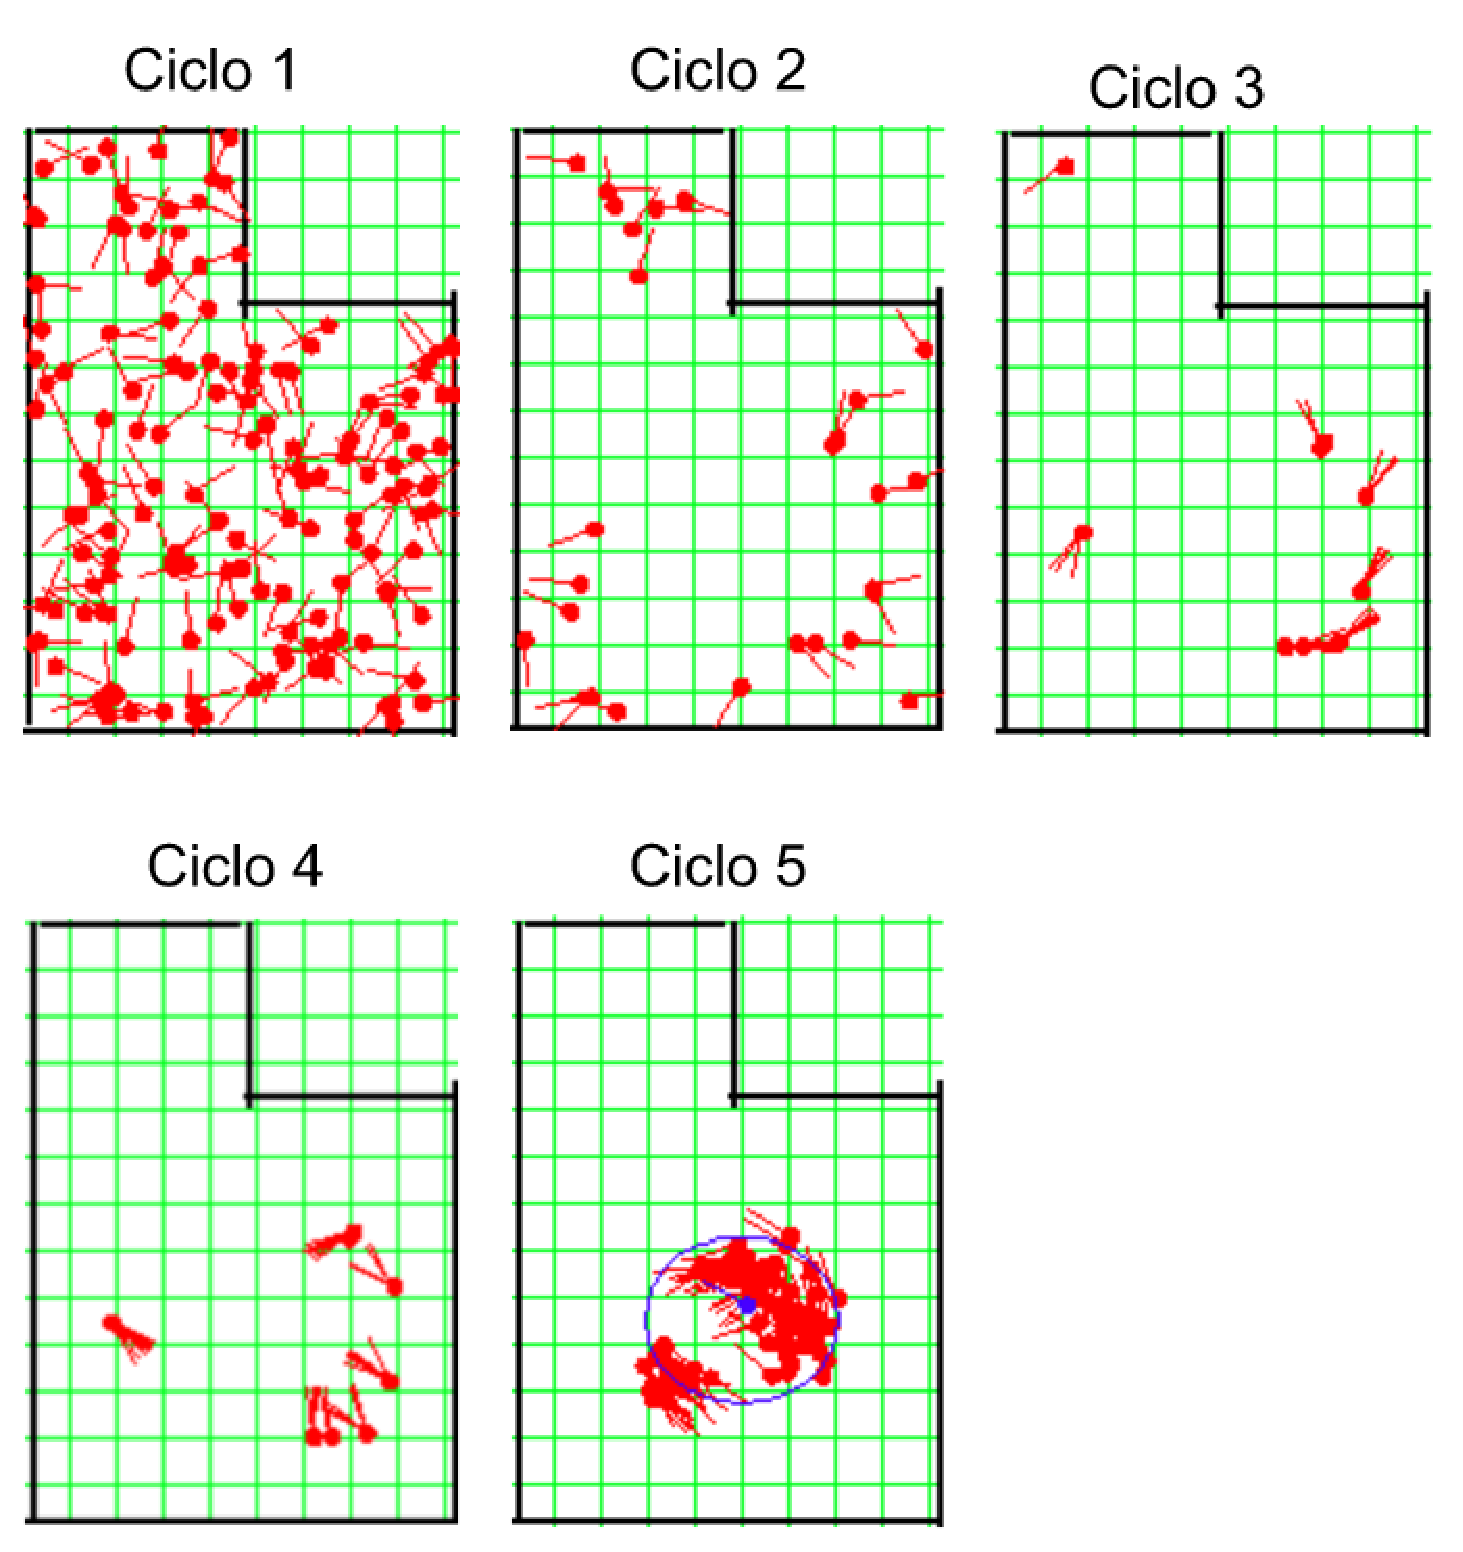
\includegraphics[scale=0.4]{figuras/cen3_ex1.eps}
  \caption[Cenário 3 - Exemplo 1]{Cenário 3 - Exemplo 1}
  \label{img:cen3_ex1}
\end{figure}


\subsection{Exemplo 2}

Exemplo utilizando velocidade de deslocamento em 5 unidades de diâmetro por segundo:

\begin{figure}[H]
  \centering
  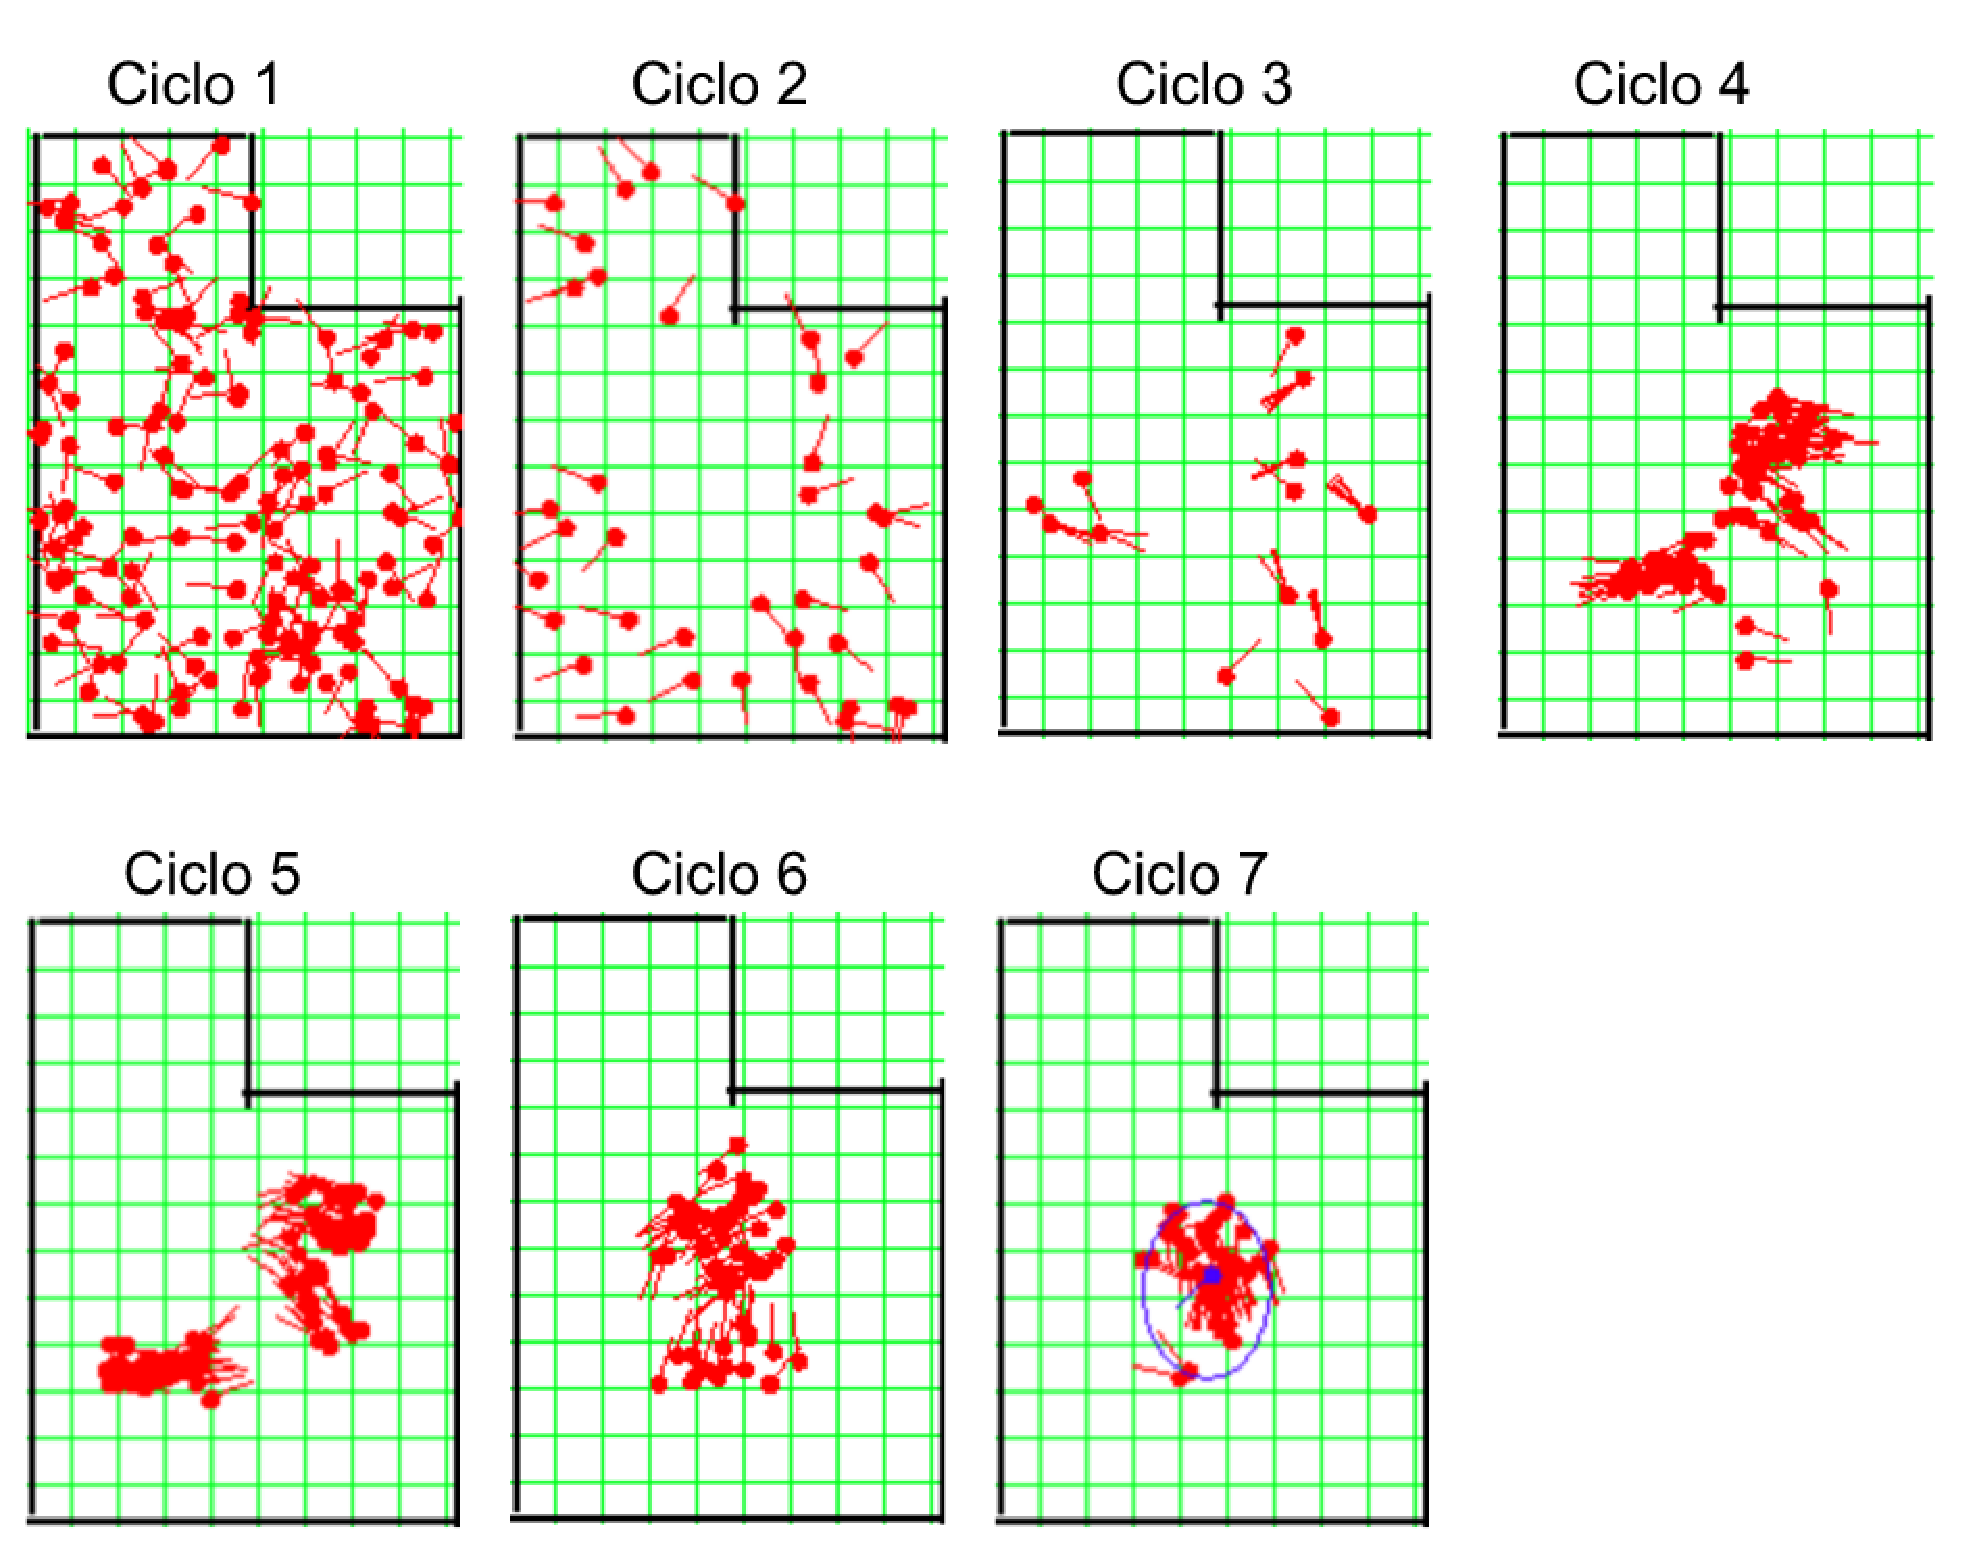
\includegraphics[scale=0.4]{figuras/cen3_ex2.eps}
  \caption[Cenário 3 - Exemplo 2]{Cenário 3 - Exemplo 2}
  \label{img:cen3_ex2}
\end{figure}


\subsection{Exemplo 3}

Exemplo utilizando velocidade de deslocamento em 10 unidades de diâmetro por segundo:

\begin{figure}[H]
  \centering
  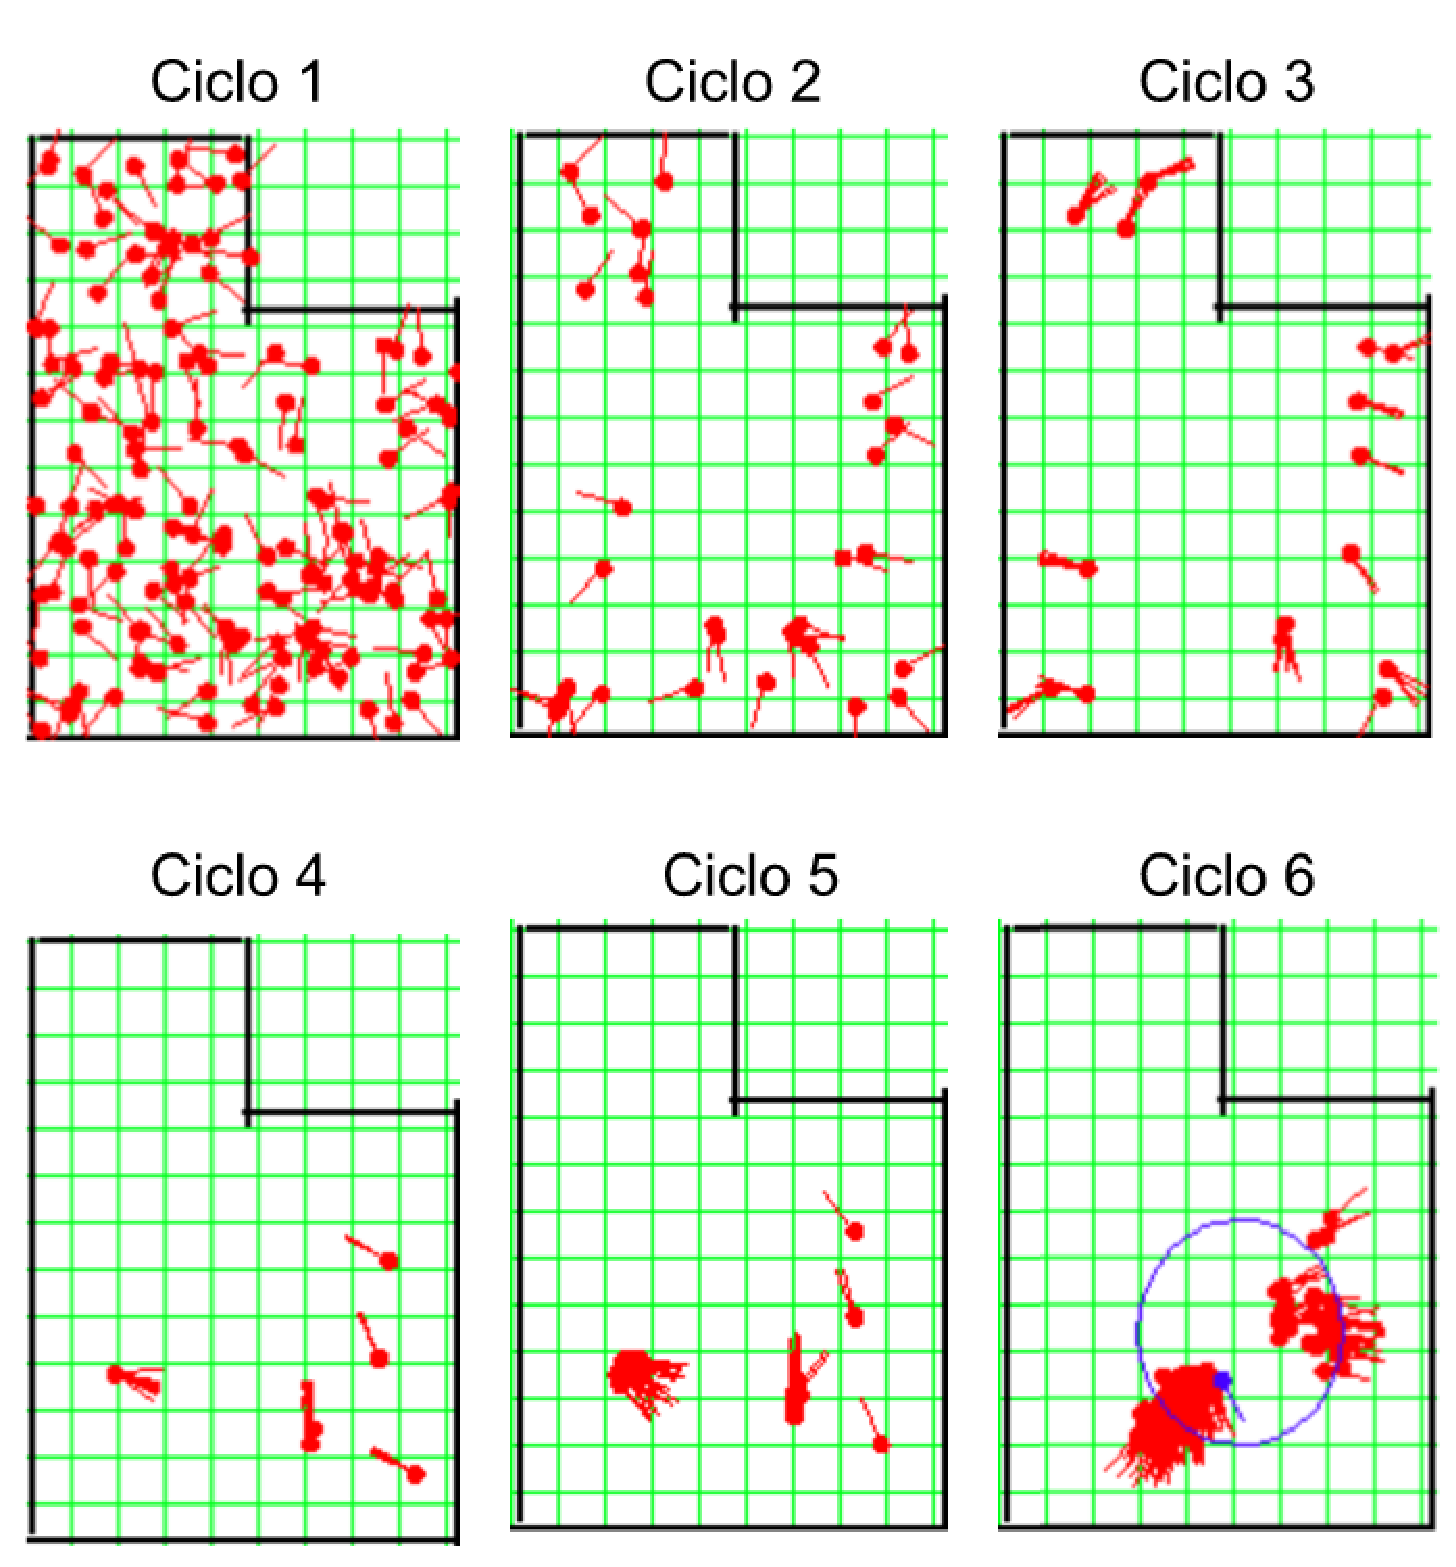
\includegraphics[scale=0.4]{figuras/cen3_ex3.eps}
  \caption[Cenário 3 - Exemplo 3]{Cenário 3 - Exemplo 3}
  \label{img:cen3_ex3}
\end{figure}

\subsection{Exemplo 4}

Exemplo utilizando velocidade de deslocamento em 15 unidades de diâmetro por segundo:

\begin{figure}[H]
  \centering
  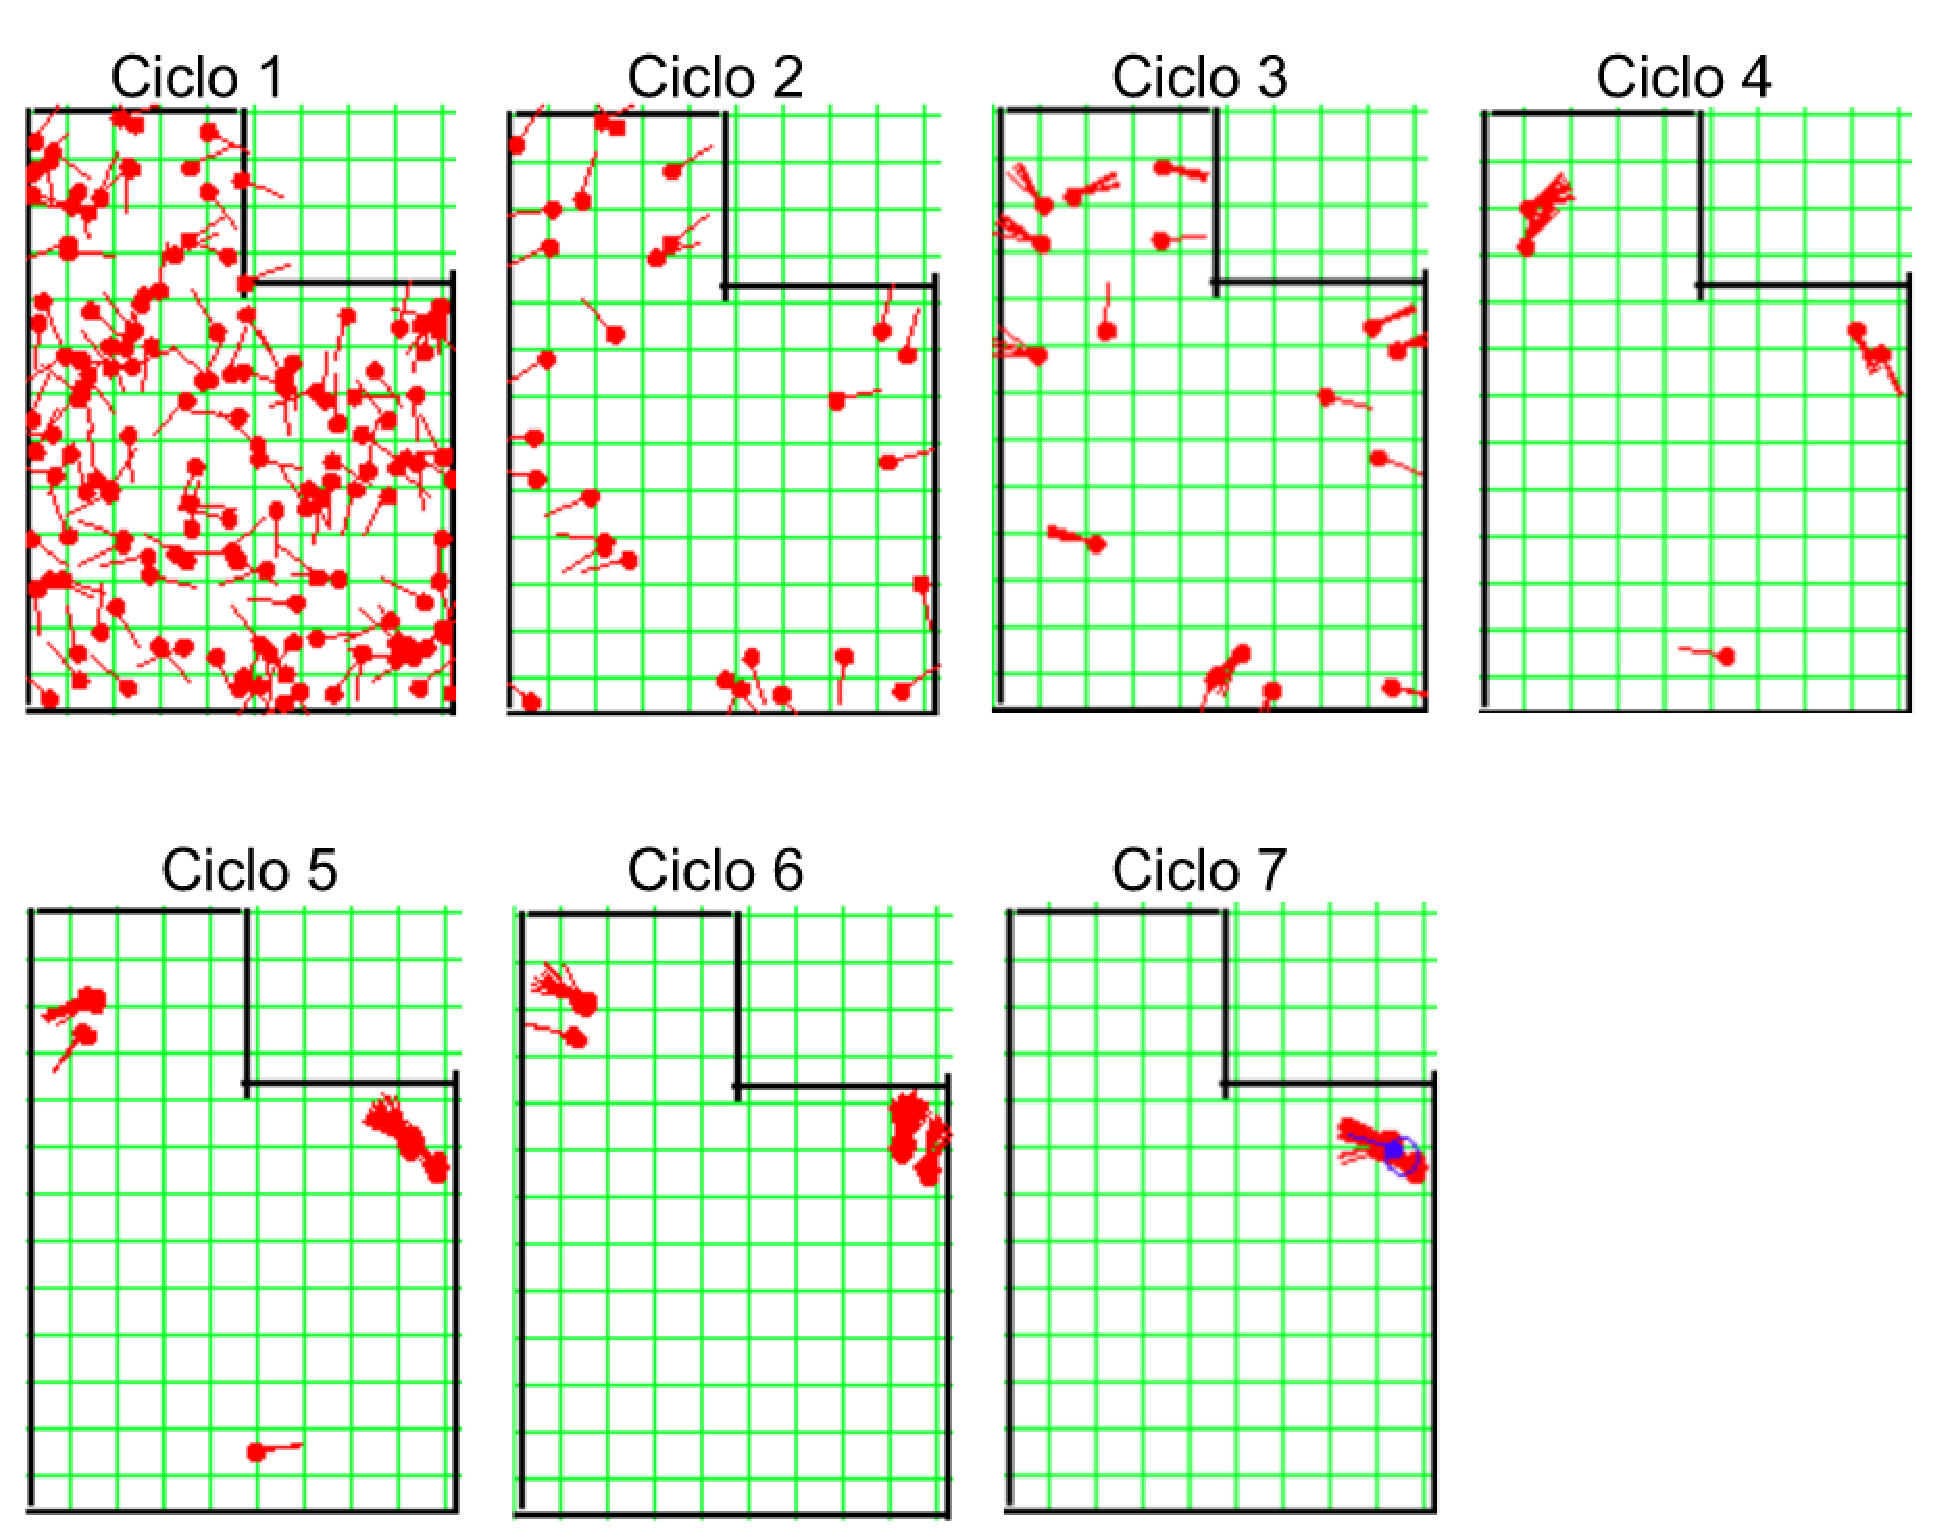
\includegraphics[scale=0.4]{figuras/cen3_ex4.eps}
  \caption[Cenário 3 - Exemplo 4]{Cenário 3 - Exemplo 4}
  \label{img:cen3_ex4}
\end{figure}

\subsection{Exemplo 5}

Exemplo utilizando velocidade de deslocamento em 30 unidades de diâmetro por segundo:

\begin{figure}[H]
  \centering
  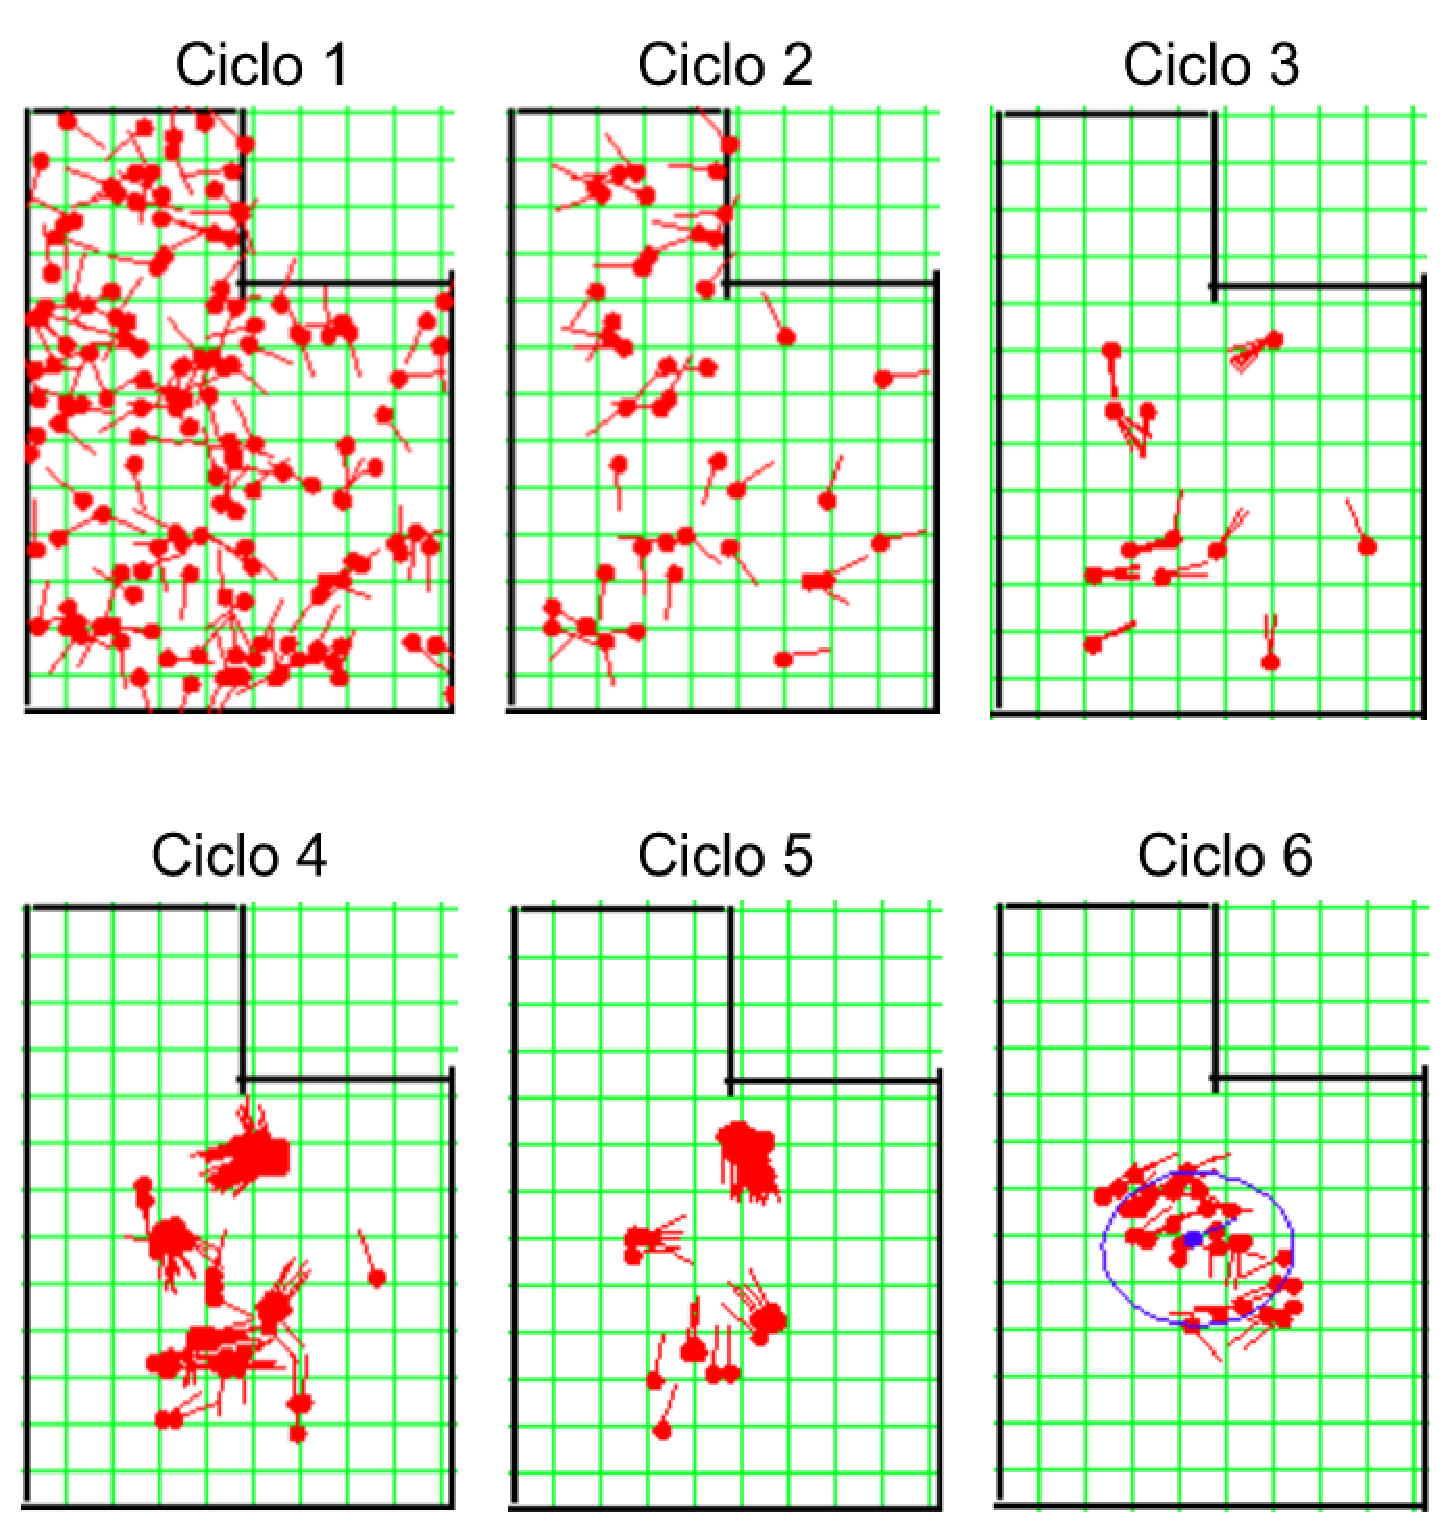
\includegraphics[scale=0.4]{figuras/cen3_ex5.eps}
  \caption[Cenário 3 - Exemplo 5]{Cenário 3 - Exemplo 5}
  \label{img:cen3_ex5}
\end{figure}
